\documentclass{article}

% packages and configurations
\usepackage{hyperref}
\usepackage{animate} % needed for animations and videos
\usepackage{bm} % bold font in equation environments
\usepackage[utf8]{inputenc}	% für Umlaute ect.
\usepackage{fancyhdr} % für header
\usepackage{lastpage} % für footer
\usepackage{extramarks} % für header und footer
\usepackage{amsthm} % math stuff
\usepackage{amsmath} % math stuff
\usepackage{amssymb} % math stuff
\usepackage{color}
\usepackage{listings} % code listings
\usepackage{graphicx} % für graphics
\usepackage[toc]{glossaries} % Glossar
\usepackage{color}
\usepackage{tikz}
\usepackage[absolute,overlay]{textpos} %to translate graphics through space
\usepackage{soul}
\usepackage{xcolor}
\usepackage{textpos}
\usepackage{caption}
\usepackage{parcolumns}
\usepackage{enumerate}
\usepackage[ngerman]{babel} % Umlaute
\usepackage[T1]{fontenc}    % this is needed for correct output of umlauts in pd
\usepackage[section]{placeins} %forces placeins to stay in section
\usepackage{datetime} % custom dates
\usepackage{afterpage}
\usepackage[section]{placeins}


\title{Building an interface between probabilistic programming languages and lumen}
\author{Jonas Aaron Gütter  \\
	Friedrich Schiller Universität Jena  \\
    Matrikelnr 152127 \\
    Prof.Dr. Joachim Giesen \\
    M. Sc. Phillip Lucas
	}

\makeglossaries


\begin{document}


\maketitle

\begin{abstract}
(1) grober Fahrplan
\begin{itemize}
   \item read related material:
        \begin{itemize}
        \item understand what Probabilistic Programming Languages (PPLs) are
        \item understand main idea of Lumen and what we want to do with it
        \item understand and formulate “why \& what”
        \end{itemize}
    \item choose a PPL
        \begin{itemize}
        \item work out requirements to chose PPL
        \item work out preferred (but not necessarily required) features
        \item chose a PPL based on these requirements and preferences
        \end{itemize}
    \item get started with PPL
    	\begin{itemize}
        \item play around, learn how to use it, what it can do, etc
              also confirm identified 'pain point', i.e. understand and
              formulate what problem you are trying to solve, why this is
              relevant and outline how you plan to solve that pain point
        \end{itemize}
    \item design a wrapper of chose PPL for Backend of Lumen
    \item give presentation about work so far, its justification, relevance, verification ideas, etc etc
    \item implement and test wrapper
    \item evaluate implementation in terms of goals set in beginning

\end{itemize}
(2) interessante PPLs:

\begin{itemize}
     \item stan for python: https://pystan.readthedocs.io/en/latest/
    \item pymc3: https://docs.pymc.io/notebooks/getting\_started.html\#Case-study-2:-Coal-mining-disasters
    \item edward: http://edwardlib.org/getting-started
    \item pyro: http://pyro.ai/
\end{itemize}
Wegen eines Arbeitsplatzes und eines PCs erkundigen wir uns.
Als Anmelde und Starttermin für Deine MA halten wir Mitte September (Mo, 17. September) im Auge.

\end{abstract}

\tableofcontents

\newglossaryentry{Bayesian network}
{
  name=Bayesian network,
  description={...}
}

\newglossaryentry{conditional probability distribution}
{
  name=conditional probability distribution,
  description={...}
}

\newglossaryentry{inference algorithm}
{
  name=inference algorithm,
  description={is a key part of a \gls{probabilistic reasoning system}}
}

\newglossaryentry{joint probability distribution}
{
  name=joint probability distribution,
  description={...}
}

\newglossaryentry{marginal distribution}
{
  name=marginal distribution,
  description={...}
}

\newglossaryentry{probabilistic model}
{
  name=probabilistic model,
  description={is a key part of a \gls{probabilistic reasoning system}}
}

\newglossaryentry{probabilistic programming}
{
  name=probabilistic programming,
  description={is something}
}

\newglossaryentry{probabilistic programming language}
{
  name=probabilistic programming language,
  description={is used to create a \gls{probabilistic reasoning system} more effectively than with a conventional programming language}
}

\newglossaryentry{probabilistic reasoning system}
{
  name=probabilistic reasoning system,
  description={consists of a \gls{probabilistic model} and an \gls{inference algorithm}}
}

\newglossaryentry{Turing-complete}
{
  name=Turing-complete,
  description={a turing-complete machine can perform any computation that could theoretically performed by any computer. universally programmable.}
}
\printglossaries
\section{Rules of Probabilistic Inference}

There are three rules of probabilistic inference: The chain rule, the total probability rule, and the Bayes' rule. The following explanations are taken from \cite{9781617292330}.

\subsection{Chain rule}

The chain rule is used to calculate a \gls{joint probability distribution} of several variables from local \gls{conditional probability distribution}s of these variables:

\begin{equation}
  P(X_1 ,X_2 ,...X_n ) = P(X_1 )P(X_2 | X_1 )P(X_3 | X_1 ,X_2 )...P(X_n | X_1 ,X_2 ,...X_{n-1}) )
\end{equation}

\subsection{Total probability rule}

The total probability rule calculates the probability distribution over a subset of variables, also called a \gls{marginal distribution}, by summing out all the other variables, that is by summing the probability distributions for each combination of values of these variables:

\begin{equation}
P(\boldsymbol X |\boldsymbol Z ) = \sum_{\boldsymbol y}   P(\boldsymbol X ,\boldsymbol Y =\boldsymbol y |\boldsymbol Z )
\end{equation} 

\subsection{Bayes' rule}

Bayes' rule calculates the probability of a cause, given aneffect, by using the prior probability of the cause and the probability of the effect, given the cause. The Bayes' rule can be derived from the chain rule.

\begin{equation}
P(X|Y) = ( P(Y|X) * P(X) ) / P(Y)
\end{equation}

\section{Bayesian models}

A Bayesian model is about assigning probabilities to model parameters. The model parameters $\beta$ themselves are considered as random variables which depend on hyperparameters $\alpha$.
\\
According to \cite{Wang2018}, the likelihood of a new datapoint can be calculated by integrating the product of the prior likelihood and conditional probability of $\beta$ over the space of $\beta$, as shown in equation \ref{eq:posterior_predictive}. This formula can also be derived using the chain rule (I think).



\begin{equation}
p(x_{new}|\boldsymbol x, \alpha) = \int p(x_{new}|\beta) * p(\beta | \boldsymbol x,\alpha) d \beta
\label{eq:posterior_predictive}
\end{equation}



\section{What is Probabilistic Programming}

Modelle spezifizieren/beschreiben 

\cite{wiki:Probabilisticprogramminglanguage}

effizienter in der Beschreibung von Modellen als herkömmliche Programmiersprachen \cite{Hardesty2015}

unifying general purpose programming with probabilistic modeling \cite{probabilistic-programming.org}


A \gls{probabilistic reasoning system} uses prior knowledge in the form of a \gls{probabilistic model} to answer a certain query. The particular propertes of the query as well as the prior knowledge are given to an \gls{inference algorithm} which returns an answer in the form of probabilities. Example is shown in figure \ref{fig:example_prs}. Probabilistic Programming is the implementation of a \gls{probabilistic reasoning system} by using a programming language.

Traditional means for representing models are not always sufficient for probabilistic models. Therefore, probabilistic programming languages were introduced to be able to represent models with the full power of a programming language (http://www.probabilistic-programming.org/wiki/Home).


\begin{figure}
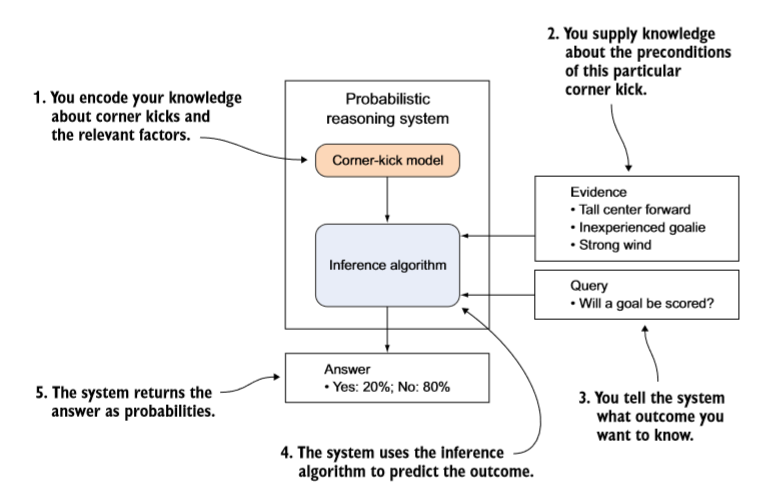
\includegraphics[width=\textwidth]{images/probabilistic_reasoning_system.PNG}
\caption[General workflow example of a probabilistic reasoning system. Source: \cite{9781617292330}]{General workflow example of a probabilistic reasoning system}
\label{fig:example_prs}
\end{figure}

% how to call a glossar entry: 

\section{Existing PPLs}

\subsection{Stan for python}

\subsection{Pymc3}

python library

fit Bayesian models, including Markov Chai Monte Carlo (MCMC) and variational inference (VI)


\subsection{Edward}

\subsection{Pyro}


\section{Lumen}

\listoffigures
        
\section{Literatur}

\bibliography{Literatur.bib}
\bibliographystyle{ieeetr}


\end{document}